\documentclass[tikz,border=10pt]{standalone}
\usepackage{tikz}
\usetikzlibrary{shapes, arrows.meta, positioning, fit, calc, backgrounds, shadows}

% --- 配色方案 ---
\definecolor{cMainFill}{RGB}{235, 245, 255} \definecolor{cMainDraw}{RGB}{33, 150, 243}
\definecolor{cFeatFill}{RGB}{255, 240, 245} \definecolor{cFeatDraw}{RGB}{233, 30, 99}
\definecolor{lineColor}{RGB}{60, 60, 60}

\tikzset{
    font=\footnotesize\sffamily,
    % --- 提交节点 ---
    commitNode/.style={
        circle, thick, draw=#1, fill=white,
        minimum size=0.65cm, inner sep=0pt,
        drop shadow={opacity=0.05},
        font=\scriptsize\bfseries
    },
    % --- 泳道标签 ---
    laneLabel/.style={
        font=\bfseries\normalsize, anchor=east, align=right
    },
    % --- 连线基础 ---
    conn/.style={
        draw=lineColor, line width=0.8pt,
        -{Latex[length=2mm, width=1.2mm]},
        font=\scriptsize\sffamily
    },
    % 虚线
    connDashed/.style={
        conn, dashed, draw=gray!70
    },
    % --- 标签样式 (优化了padding和背景) ---
    cmdLabel/.style={
        midway, 
        fill=white,          % 白色背景遮挡底下的线
        text=lineColor, 
        inner sep=2.5pt,     % 稍微增加内边距,呼吸感更强
        rounded corners=3pt,
        align=center, 
        font=\scriptsize\ttfamily,
        fill opacity=0.9,    % 背景微透,不至于太生硬
        text opacity=1,
        drop shadow={opacity=0.05}
    }
}

\begin{document}
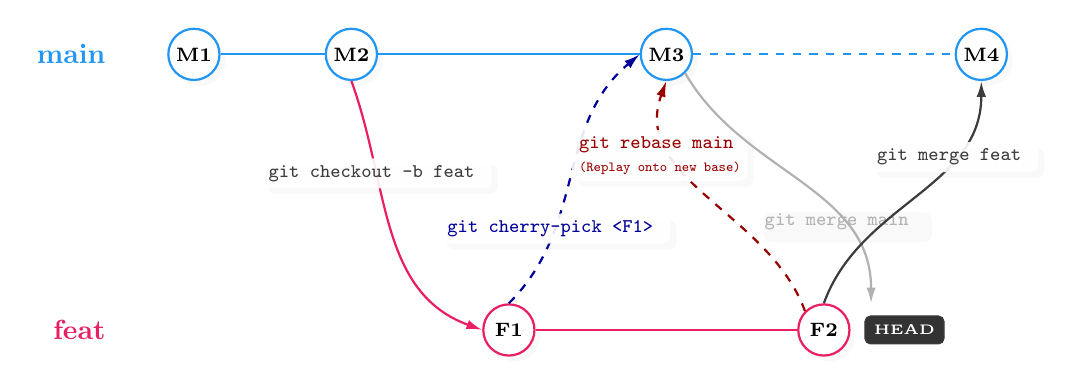
\begin{tikzpicture}[node distance=1.5cm and 1.5cm]

	% =========================================
	% 1. 布局骨架 (拉大坐标间距)
	% =========================================

	% --- Main Branch (Top, y=0) ---
	\node[laneLabel, text=cMainDraw] at (-1, 0) {main};

	% 坐标拉开:0 -> 2 -> 6 -> 10
	\node[commitNode=cMainDraw] (m1) at (0, 0) {M1};
	\node[commitNode=cMainDraw] (m2) at (2.0, 0) {M2};
	\node[commitNode=cMainDraw] (m3) at (6.0, 0) {M3};
	\node[commitNode=cMainDraw] (m4) at (10.0, 0) {M4};

	\draw[thick, cMainDraw] (m1) -- (m2) -- (m3);
	\draw[thick, cMainDraw, dashed] (m3) -- (m4);

	% --- Feature Branch (Bottom, y=-3.5) ---
	% 【关键修改】:y从-2.0改为-3.5,拉开垂直距离
	\node[laneLabel, text=cFeatDraw] at (-1, -3.5) {feat};

	% 坐标错位:F1在M2和M3之间,F2在M3和M4之间
	\node[commitNode=cFeatDraw] (f1) at (4.0, -3.5) {F1};
	\node[commitNode=cFeatDraw] (f2) at (8.0, -3.5) {F2};

	\draw[thick, cFeatDraw] (f1) -- (f2);

	% =========================================
	% 2. 连线与指令 (交错布局)
	% =========================================

	% 1. [Checkout]: M2 -> F1
	% 放在左侧,空间充裕
	\draw[conn, cFeatDraw, thick] (m2.south) to[out=290, in=160]
	node[cmdLabel, pos=0.3] {
		git checkout -b feat
	}
	(f1.west);

	% 2. [Cherry-pick]: F1 -> M3 (斜向右上)
	\draw[connDashed, blue!60!black] (f1.north) to[out=45, in=220]
	node[cmdLabel, pos=0.3, text=blue!60!black] {
		git cherry-pick <F1>
	}
	(m3.west);

	% 3. [Rebase]: F2 -> M3 (红色虚线)
	\draw[connDashed, red!60!black] (f2.north west) to[out=110, in=250]
    node[cmdLabel, pos=0.7, text=red!60!black, align=left, xshift=-5pt] {
        git rebase main\\
        \tiny (Replay onto new base)
    }
    (m3.south);

	% 4. [Merge Main]: M3 -> F2 (灰色实线)
	\draw[conn, gray!60] (m3.south east) to[out=300, in=90]
	node[cmdLabel, pos=0.7, text=gray!60, fill=none] {
		git merge main
	}
	($(f2.north)+(0.6,0)$);

	% 5. [Merge Feat]: F2 -> M4
	\draw[conn, thick] (f2.north) to[out=70, in=270]
	node[cmdLabel, pos=0.7] {
		git merge feat
	}
	(m4.south);

	% HEAD 标记
	\node[draw=lineColor, fill=black!80, text=white, rounded corners=2pt, font=\tiny\bfseries, right=5pt of f2] {HEAD};

\end{tikzpicture}
\end{document}